% Options for packages loaded elsewhere
\PassOptionsToPackage{unicode}{hyperref}
\PassOptionsToPackage{hyphens}{url}
%
\documentclass[
]{article}
\usepackage{amsmath,amssymb}
\usepackage{iftex}
\ifPDFTeX
  \usepackage[T1]{fontenc}
  \usepackage[utf8]{inputenc}
  \usepackage{textcomp} % provide euro and other symbols
\else % if luatex or xetex
  \usepackage{unicode-math} % this also loads fontspec
  \defaultfontfeatures{Scale=MatchLowercase}
  \defaultfontfeatures[\rmfamily]{Ligatures=TeX,Scale=1}
\fi
\usepackage{lmodern}
\ifPDFTeX\else
  % xetex/luatex font selection
\fi
% Use upquote if available, for straight quotes in verbatim environments
\IfFileExists{upquote.sty}{\usepackage{upquote}}{}
\IfFileExists{microtype.sty}{% use microtype if available
  \usepackage[]{microtype}
  \UseMicrotypeSet[protrusion]{basicmath} % disable protrusion for tt fonts
}{}
\makeatletter
\@ifundefined{KOMAClassName}{% if non-KOMA class
  \IfFileExists{parskip.sty}{%
    \usepackage{parskip}
  }{% else
    \setlength{\parindent}{0pt}
    \setlength{\parskip}{6pt plus 2pt minus 1pt}}
}{% if KOMA class
  \KOMAoptions{parskip=half}}
\makeatother
\usepackage{xcolor}
\usepackage[margin=1in]{geometry}
\usepackage{longtable,booktabs,array}
\usepackage{calc} % for calculating minipage widths
% Correct order of tables after \paragraph or \subparagraph
\usepackage{etoolbox}
\makeatletter
\patchcmd\longtable{\par}{\if@noskipsec\mbox{}\fi\par}{}{}
\makeatother
% Allow footnotes in longtable head/foot
\IfFileExists{footnotehyper.sty}{\usepackage{footnotehyper}}{\usepackage{footnote}}
\makesavenoteenv{longtable}
\usepackage{graphicx}
\makeatletter
\def\maxwidth{\ifdim\Gin@nat@width>\linewidth\linewidth\else\Gin@nat@width\fi}
\def\maxheight{\ifdim\Gin@nat@height>\textheight\textheight\else\Gin@nat@height\fi}
\makeatother
% Scale images if necessary, so that they will not overflow the page
% margins by default, and it is still possible to overwrite the defaults
% using explicit options in \includegraphics[width, height, ...]{}
\setkeys{Gin}{width=\maxwidth,height=\maxheight,keepaspectratio}
% Set default figure placement to htbp
\makeatletter
\def\fps@figure{htbp}
\makeatother
\setlength{\emergencystretch}{3em} % prevent overfull lines
\providecommand{\tightlist}{%
  \setlength{\itemsep}{0pt}\setlength{\parskip}{0pt}}
\setcounter{secnumdepth}{5}
\ifLuaTeX
  \usepackage{selnolig}  % disable illegal ligatures
\fi
\usepackage{bookmark}
\IfFileExists{xurl.sty}{\usepackage{xurl}}{} % add URL line breaks if available
\urlstyle{same}
\hypersetup{
  pdftitle={HarvardX: PH125.9x Data Science - EDX Project: Choose Your Own},
  pdfauthor={Matias Ezequiel Maurig},
  hidelinks,
  pdfcreator={LaTeX via pandoc}}

\title{HarvardX: PH125.9x Data Science - EDX Project: Choose Your Own}
\author{Matias Ezequiel Maurig}
\date{2024-11-16}

\begin{document}
\maketitle

{
\setcounter{tocdepth}{3}
\tableofcontents
}
\newpage

\section{Predicting Diabetes Onset: A Machine Learning
Approach}\label{predicting-diabetes-onset-a-machine-learning-approach}

\subsection{Introduction}\label{introduction}

The Pima Indians Diabetes Database is a well-known dataset from Kaggle
used to predict the onset of diabetes based on various diagnostic
measures. This dataset originally comes from the National Institute of
Diabetes and Digestive and Kidney Diseases, and its primary objective is
to classify individuals as either diabetic or non-diabetic based on
their medical and diagnostic information.

Diabetes is one of the most widespread diseases globally, with an
estimated 9.3\% of the world population affected by diabetes. In
particular, type 2 diabetes is a major health concern and is often
preventable through early intervention. The Pima Indians Diabetes
dataset provides a valuable opportunity to apply machine learning
algorithms to improve the accuracy and efficiency of predicting
diabetes, enabling healthcare professionals to make earlier and more
informed decisions.

\subsection{Project Overview}\label{project-overview}

This project is part of the HarvardX PH125.9x Data Science: Capstone
course, where our objective is to develop a machine learning model to
predict the onset of diabetes. The project, titled ``Choose Your Own,''
provides the flexibility to explore and experiment with different
methodologies, focusing on training and comparing various models to
determine the most effective one.

In this project, we will:

\emph{Preprocess and clean the dataset:} Handle missing values, scale
the data, and prepare it for modeling. \emph{Train multiple
classification models:} We will experiment with different algorithms and
techniques to predict whether a person is diabetic based on diagnostic
measures. \emph{Compare model performance:} After training the models,
we will evaluate them using various performance metrics, such as
accuracy, precision, recall, and AUC-ROC, to identify the most effective
model for predicting diabetes. \emph{Select the best model:} By
comparing the results from different models, we will choose the one that
offers the best balance of predictive power and efficiency for
real-world application.

The goal is to find the most accurate and reliable model that can
predict the onset of diabetes, enabling earlier diagnosis and
intervention.

\subsubsection{Goal of the Project}\label{goal-of-the-project}

The goal of this project is to develop and compare various machine
learning models to predict the onset of diabetes. We aim to explore
different classification algorithms and assess their performance in
accurately identifying whether a person is at risk of diabetes based on
diagnostic measures. By evaluating multiple models, we seek to determine
the most effective one for early detection, which can later be applied
to new, unseen data.

\subsubsection{Importance of Early
Detection}\label{importance-of-early-detection}

Early detection of diabetes is critical for preventing long-term
complications and improving patients' quality of life. The global
prevalence of diabetes is rising, with an estimated 9.3\% of the world's
population affected, according to the World Health Organization. By
identifying individuals at risk early, we can implement lifestyle
changes and medical interventions that may delay or even prevent the
onset of the disease. In this project, we are focusing on training
models that will assist in this early diagnosis, ultimately contributing
to better healthcare outcomes.

\section{Let's Begin with Data Analysis and
Wrangling}\label{lets-begin-with-data-analysis-and-wrangling}

\subsection{Insights About Diabetes}\label{insights-about-diabetes}

In this section, we will apply data analysis and wrangling tools to
explore the dataset. The goal is to uncover interesting patterns and
insights that may not be immediately obvious. Through data cleaning,
manipulation, and visualization, we'll start to ``surf'' through the
data and highlight key findings that help us understand the underlying
trends and factors contributing to diabetes risk. This process will
allow us to transform raw data into actionable insights, which will
guide the development of our machine learning models.

\subsection{Exploring the Relationship Between
Variables}\label{exploring-the-relationship-between-variables}

As mentioned earlier, diabetes is a disease that affects a significant
portion of the global population, with millions of people diagnosed each
year. In this section, we will dive into the dataset to explore the
relationships between different variables. Our goal is to identify how
factors such as age, glucose levels, and insulin resistance relate to
the likelihood of developing diabetes. By analyzing these variables, we
aim to uncover meaningful patterns that could enhance our predictive
models and improve early detection strategies for diabetes.

Let's start with a very global look at the structure presented by the
Kaggle data set, ``Pima Indians Diabetes Database''

\begin{verbatim}
##   Pregnancies Glucose BloodPressure SkinThickness Insulin  BMI
## 1           6     148            72            35       0 33.6
## 2           1      85            66            29       0 26.6
## 3           8     183            64             0       0 23.3
## 4           1      89            66            23      94 28.1
## 5           0     137            40            35     168 43.1
##   DiabetesPedigreeFunction Age Outcome
## 1                    0.627  50       1
## 2                    0.351  31       0
## 3                    0.672  32       1
## 4                    0.167  21       0
## 5                    2.288  33       1
\end{verbatim}

\begin{verbatim}
## 'data.frame':    768 obs. of  9 variables:
##  $ Pregnancies             : int  6 1 8 1 0 5 3 10 2 8 ...
##  $ Glucose                 : int  148 85 183 89 137 116 78 115 197 125 ...
##  $ BloodPressure           : int  72 66 64 66 40 74 50 0 70 96 ...
##  $ SkinThickness           : int  35 29 0 23 35 0 32 0 45 0 ...
##  $ Insulin                 : int  0 0 0 94 168 0 88 0 543 0 ...
##  $ BMI                     : num  33.6 26.6 23.3 28.1 43.1 25.6 31 35.3 30.5 0 ...
##  $ DiabetesPedigreeFunction: num  0.627 0.351 0.672 0.167 2.288 ...
##  $ Age                     : int  50 31 32 21 33 30 26 29 53 54 ...
##  $ Outcome                 : int  1 0 1 0 1 0 1 0 1 1 ...
\end{verbatim}

\newpage

\subsection{Dataset Structure and
Variables}\label{dataset-structure-and-variables}

The dataset is structured with several columns, each representing a
specific diagnostic measurement or demographic detail of individuals.
Let's look at each one a little more in depth.:

\begin{itemize}
\tightlist
\item
  \textbf{Pregnancies}: The number of times the individual has been
  pregnant.\\
\item
  \textbf{Glucose}: Plasma glucose concentration measured during an oral
  glucose tolerance test.\\
\item
  \textbf{BloodPressure}: Diastolic blood pressure (mm Hg).\\
\item
  \textbf{SkinThickness}: Triceps skinfold thickness (mm).\\
\item
  \textbf{Insulin}: 2-hour serum insulin (mu U/ml).\\
\item
  \textbf{BMI}: Body Mass Index, calculated as weight in kg divided by
  the square of height in meters.\\
\item
  \textbf{DiabetesPedigreeFunction}: A function that scores the
  likelihood of diabetes based on family history and genetic factors.\\
\item
  \textbf{Age}: The age of the individual (years).\\
\item
  \textbf{Outcome}: A binary variable indicating whether the individual
  has diabetes (1) or not (0).\\
\item
  \textbf{HighInsulin}: An additional feature created for analysis,
  indicating high insulin levels.
\end{itemize}

This dataset provides a range of medical and demographic details that
can help us understand the relationships between these variables and
diabetes occurrence. By exploring and analyzing these features, we aim
to uncover patterns that could improve predictive accuracy in
determining diabetes outcomes.

\begin{verbatim}
## 
##   0   1 
## 500 268
\end{verbatim}

\begin{center}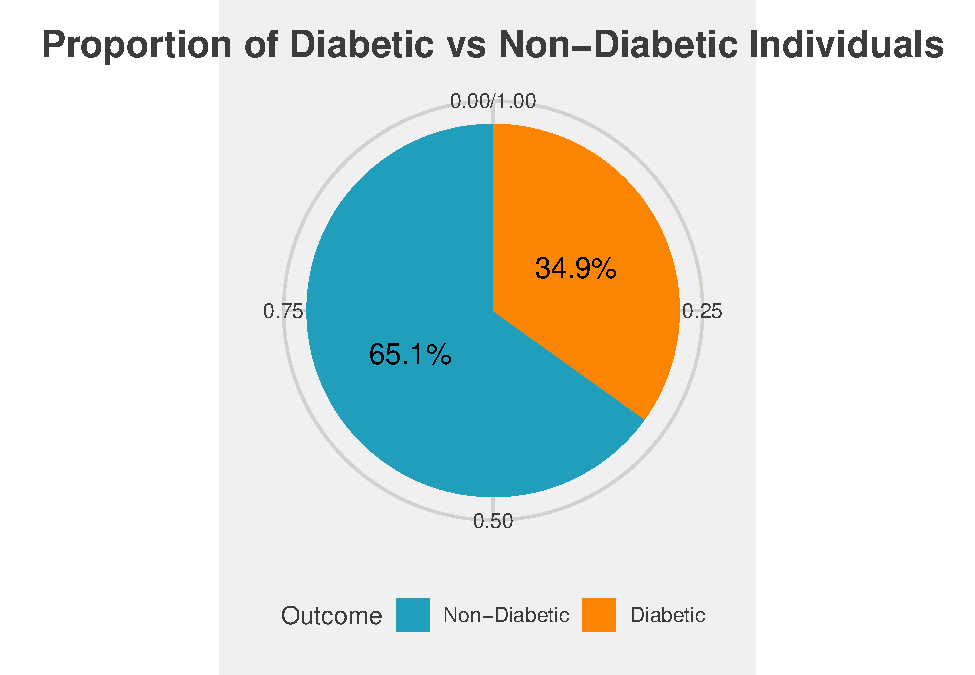
\includegraphics{Diabetes-Project_files/figure-latex/outcomes-1} \end{center}

The dataset includes a total of \textbf{768 records}, divided into two
groups based on the \textbf{Outcome} variable:

\begin{itemize}
\tightlist
\item
  \textbf{500 individuals (65.1\%)} do not have diabetes (Outcome =
  0).\\
\item
  \textbf{268 individuals (34.9\%)} have diabetes (Outcome = 1).
\end{itemize}

\section{Correlation Analysis}\label{correlation-analysis}

To explore relationships among variables, we calculated the correlation
matrix for the dataset. Here are some notable correlations:

\begin{verbatim}
## # A tibble: 2 x 9
##   Outcome Age_mean Age_sd Glucose_mean Glucose_sd BMI_mean BMI_sd Insulin_mean
##     <int>    <dbl>  <dbl>        <dbl>      <dbl>    <dbl>  <dbl>        <dbl>
## 1       0     31.2   11.7         110.       26.1     30.3   7.69         68.8
## 2       1     37.1   11.0         141.       31.9     35.1   7.26        100. 
## # i 1 more variable: Insulin_sd <dbl>
\end{verbatim}

\begin{verbatim}
##                          Pregnancies    Glucose BloodPressure SkinThickness
## Pregnancies               1.00000000 0.12945867    0.14128198   -0.08167177
## Glucose                   0.12945867 1.00000000    0.15258959    0.05732789
## BloodPressure             0.14128198 0.15258959    1.00000000    0.20737054
## SkinThickness            -0.08167177 0.05732789    0.20737054    1.00000000
## Insulin                  -0.07353461 0.33135711    0.08893338    0.43678257
## BMI                       0.01768309 0.22107107    0.28180529    0.39257320
## DiabetesPedigreeFunction -0.03352267 0.13733730    0.04126495    0.18392757
## Age                       0.54434123 0.26351432    0.23952795   -0.11397026
## Outcome                   0.22189815 0.46658140    0.06506836    0.07475223
##                              Insulin        BMI DiabetesPedigreeFunction
## Pregnancies              -0.07353461 0.01768309              -0.03352267
## Glucose                   0.33135711 0.22107107               0.13733730
## BloodPressure             0.08893338 0.28180529               0.04126495
## SkinThickness             0.43678257 0.39257320               0.18392757
## Insulin                   1.00000000 0.19785906               0.18507093
## BMI                       0.19785906 1.00000000               0.14064695
## DiabetesPedigreeFunction  0.18507093 0.14064695               1.00000000
## Age                      -0.04216295 0.03624187               0.03356131
## Outcome                   0.13054795 0.29269466               0.17384407
##                                  Age    Outcome
## Pregnancies               0.54434123 0.22189815
## Glucose                   0.26351432 0.46658140
## BloodPressure             0.23952795 0.06506836
## SkinThickness            -0.11397026 0.07475223
## Insulin                  -0.04216295 0.13054795
## BMI                       0.03624187 0.29269466
## DiabetesPedigreeFunction  0.03356131 0.17384407
## Age                       1.00000000 0.23835598
## Outcome                   0.23835598 1.00000000
\end{verbatim}

\begin{itemize}
\tightlist
\item
  \textbf{Glucose and Outcome (0.4666):} Individuals with higher glucose
  levels are more likely to have diabetes.\\
\item
  \textbf{BMI and Outcome (0.2927):} Higher BMI is moderately associated
  with a higher likelihood of diabetes.\\
\item
  \textbf{Pregnancies and Age (0.5443):} As expected, older individuals
  tend to have had more pregnancies.\\
\item
  \textbf{Skin Thickness and Insulin (0.4368):} These variables are
  strongly related, likely reflecting metabolic or physiological
  factors.
\end{itemize}

These insights provide initial evidence of how certain variables relate
to diabetes onset. Later, we will visualize these relationships more
effectively using graphical methods to deepen our understanding and
guide feature selection.

\subsubsection{Distribution of BMI Among Diabetic Patients by Age
Group}\label{distribution-of-bmi-among-diabetic-patients-by-age-group}

\begin{center}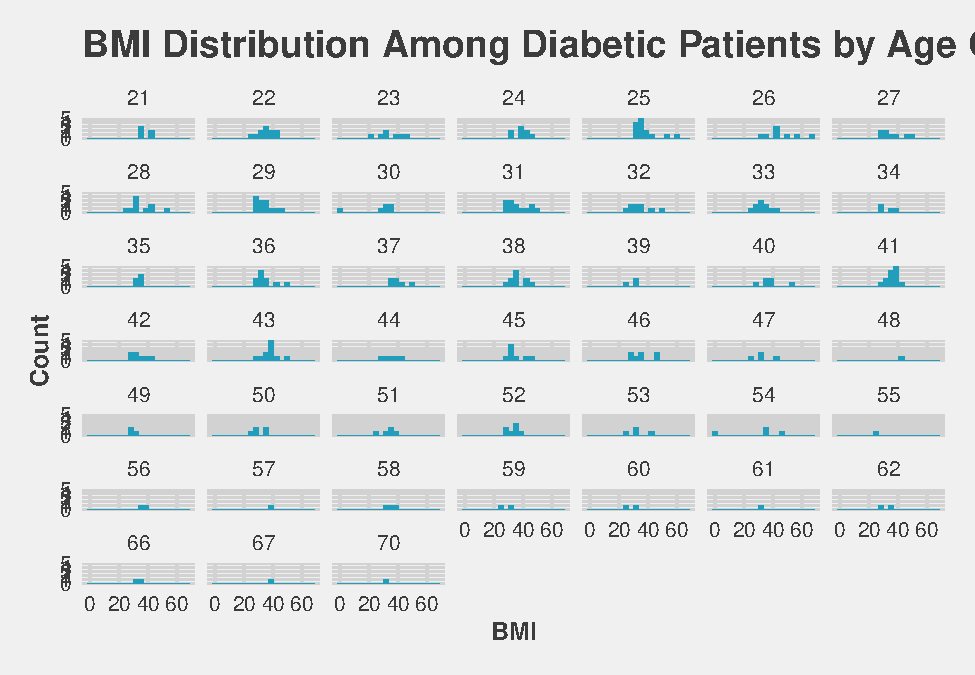
\includegraphics{Diabetes-Project_files/figure-latex/BMI vs Age-1} \end{center}

The chart reveals how Body Mass Index (BMI) varies across different age
groups for diabetic patients. As age increases, we observe notable
shifts in the BMI distribution:

\begin{itemize}
\tightlist
\item
  \textbf{Younger Age Groups}: Patients around 21 years old tend to show
  a distribution skewed towards lower BMI values, indicating that
  younger diabetic individuals are more likely to have a lower BMI
  compared to older groups.\\
\item
  \textbf{Older Age Groups}: In contrast, older diabetic patients
  display a wider and more evenly distributed range of BMI values,
  suggesting a higher prevalence of obesity or overweight conditions in
  these groups.
\end{itemize}

This trend could point to the combined effects of aging and lifestyle
changes over time, factors often linked to higher BMI among older
individuals with diabetes. This relationship will be explored further
with visual and statistical analyses.

\newpage

\subsubsection{Proportion of Diabetic Patients with Elevated Insulin
Levels}\label{proportion-of-diabetic-patients-with-elevated-insulin-levels}

The bar chart visualizes the proportion of diabetic patients with
elevated insulin levels. Elevated insulin levels are classified as
``High Insulin'' for values greater than 100, and ``Normal Insulin'' for
values at or below 100.

\begin{center}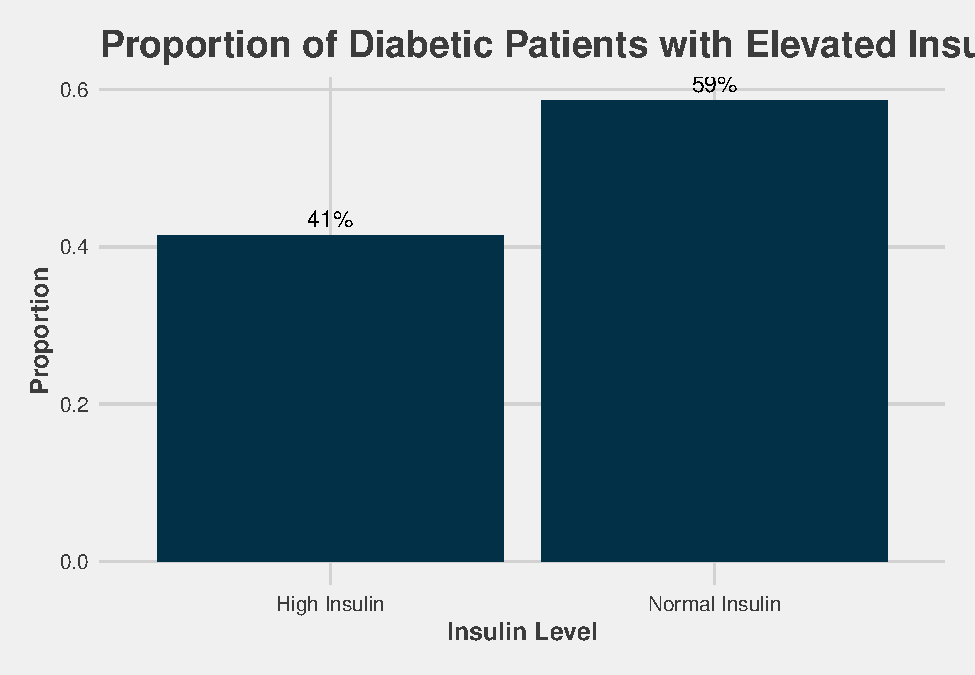
\includegraphics{Diabetes-Project_files/figure-latex/Insulin levels-1} \end{center}

\begin{itemize}
\tightlist
\item
  \textbf{High Insulin}: 41\% of diabetic patients have elevated insulin
  levels, indicating a common pattern in the diabetic population.
\item
  \textbf{Normal Insulin}: The remaining 59\% of diabetic patients have
  insulin levels within the normal range, suggesting that not all
  diabetes cases are associated with insulin resistance.
\end{itemize}

These proportions highlight the distribution of insulin levels among
diabetic patients, providing insights into the variability of insulin
resistance in the population.

\subsection{Distribution of Diabetes by Age
Group}\label{distribution-of-diabetes-by-age-group}

\begin{center}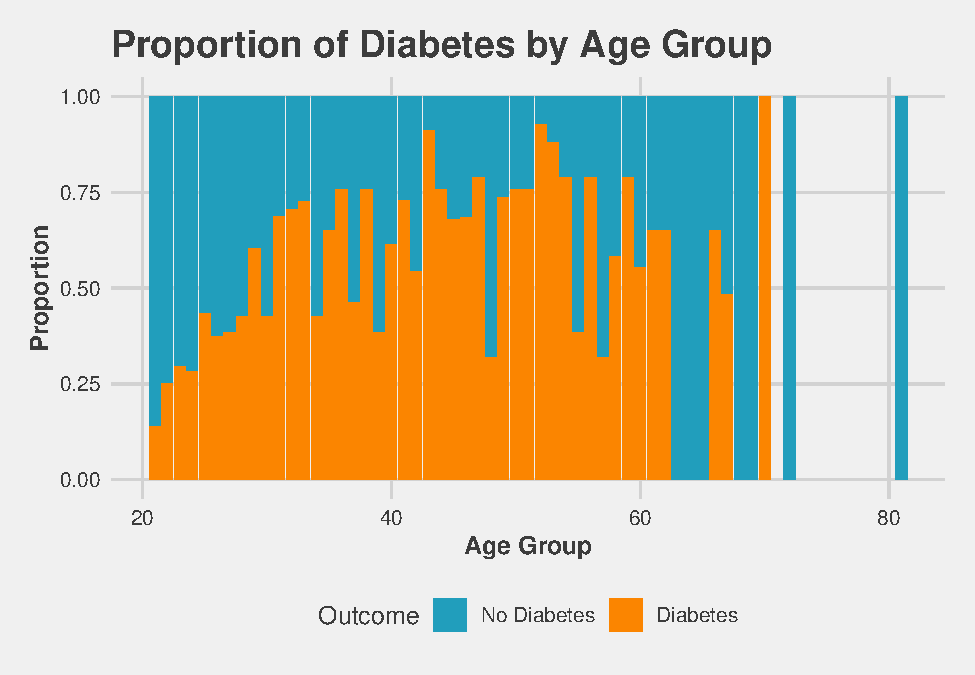
\includegraphics{Diabetes-Project_files/figure-latex/diabetes by age-1} \end{center}

The chart presents two sets of bars: one in blue representing the
proportion of individuals without diabetes and the other in red
representing the proportion with diabetes. As age increases, the
proportion of individuals with diabetes also increases, which is
reflected in the growing height of the red bars compared to the blue
bars as we move to the right along the x-axis. This chart clearly shows
how the prevalence of diabetes varies with age, indicating that diabetes
is more common in older age groups.

\subsubsection{Scatter Plot of Age vs
Glucose}\label{scatter-plot-of-age-vs-glucose}

\begin{center}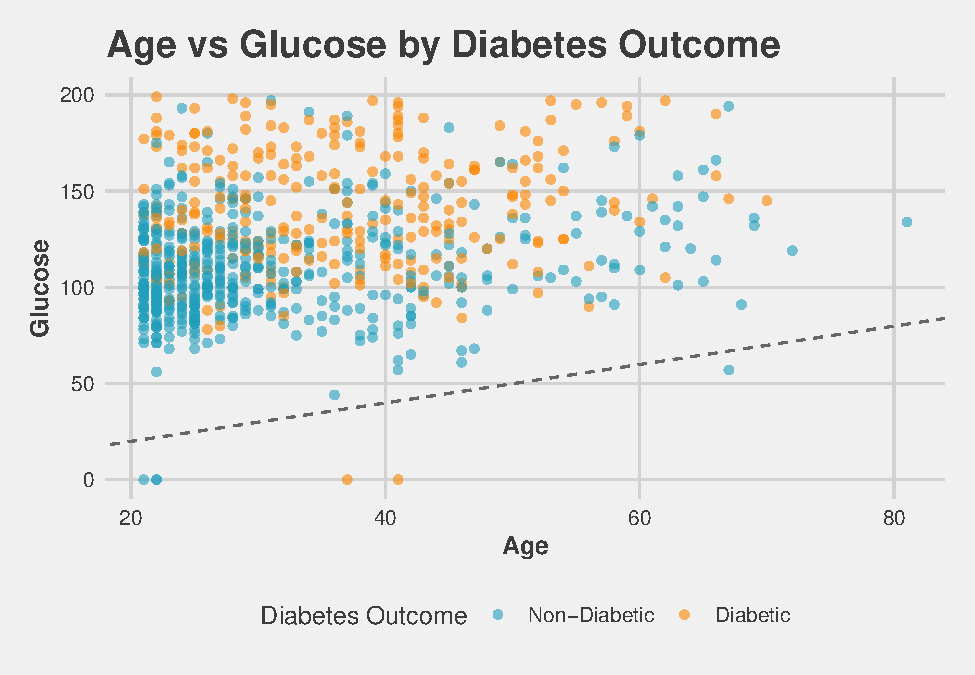
\includegraphics{Diabetes-Project_files/figure-latex/age vs glucose-1} \end{center}

As age increases, the proportion of individuals with diabetes also
increases, which is reflected in the growing height of the red bars
compared to the blue bars as we move to the right along the x-axis. This
graph suggests that diabetes is more common in older age groups. It is
important to consider these findings when designing strategies for
diabetes prevention and management based on the patient's age. People
with diabetes can monitor their blood glucose levels using a glucose
meter or a continuous glucose monitor. Regular tracking of results is
essential to assess the body's response to the diabetes care plan.

We have gathered valuable insights from the dataset by exploring the
distribution of key variables and their relationships. Next, we will
build and compare several classification models to predict diabetes,
evaluating their performance to determine which one yields the best
results.

\newpage

\section{Building Classification
Models}\label{building-classification-models}

\subsection{K-Nearest Neighbors (KNN)
Model}\label{k-nearest-neighbors-knn-model}

The first model we will use is the K-Nearest Neighbors (KNN) algorithm.
KNN is a simple, non-parametric method used for classification tasks. It
works by finding the `k' nearest data points (neighbors) to a given
point and predicting the class label based on the majority class among
these neighbors. The value of `k' is a hyperparameter that we can adjust
to optimize the model's performance.

For each model, we will use confusion matrices to assess their
performance. A confusion matrix is a tool used to measure the accuracy
of a classification model by comparing the predicted labels against the
actual labels. It shows the number of correct and incorrect predictions,
broken down by class. By evaluating the confusion matrix, we can gain
insights into how well the model distinguishes between the different
classes and calculate performance metrics such as accuracy, precision,
recall, and F1-score.

We selected \textbf{k=17} for this KNN model because, after testing
different values of kk, it provided the best overall performance. This
was determined by evaluating metrics such as accuracy and the balance
between sensitivity and specificity during cross-validation. A lower
\textbf{k} might be \emph{more sensitive} to noise, while a higher
\textbf{k} could overly \emph{smooth predictions}. With \textbf{k=17},
the model achieves a \emph{good balance}, making it more reliable for
classifying the data.

\subsubsection{KNN Confusion Matrix}\label{knn-confusion-matrix}

The confusion matrix below shows the results of the KNN model's
predictions. Here's how to interpret each part:

\begin{verbatim}
##       Predicted
## Actual  0  1
##      0 99 14
##      1 16 24
\end{verbatim}

The \textbf{confusion matrix} for the KNN model provides an overview of
the predictions made compared to the actual outcomes:

\begin{longtable}[]{@{}lll@{}}
\toprule\noalign{}
\textbf{Predicted} & \textbf{0} & \textbf{1} \\
\midrule\noalign{}
\endhead
\bottomrule\noalign{}
\endlastfoot
\textbf{Actual 0} & 99 & 14 \\
\textbf{Actual 1} & 16 & 24 \\
\end{longtable}

\begin{itemize}
\tightlist
\item
  \textbf{Correct Predictions}:

  \begin{itemize}
  \tightlist
  \item
    99 samples of class \textbf{0} were correctly classified as
    \textbf{0}.
  \item
    24 samples of class \textbf{1} were correctly classified as
    \textbf{1}.
  \end{itemize}
\item
  \textbf{Misclassifications}:

  \begin{itemize}
  \tightlist
  \item
    14 samples of class \textbf{0} were misclassified as \textbf{1}.
  \item
    16 samples of class \textbf{1} were misclassified as \textbf{0}.
  \end{itemize}
\end{itemize}

\newpage

\subsubsection{KNN Metrics}\label{knn-metrics}

Let's move on to the \textbf{metrics.} :

\begin{verbatim}
##              Metric     Value
## 1          Accuracy 0.8039216
## 2         Precision 0.8761062
## 3            Recall 0.8608696
## 4          F1-Score 0.8684211
## 5       Specificity 0.6000000
## 6 Balanced Accuracy 0.7304348
\end{verbatim}

\begin{itemize}
\tightlist
\item
  \textbf{Accuracy}: At \textbf{80.4\%}, the model is correctly
  classifying most samples.
\item
  \textbf{Precision}: With a value of \textbf{87.6\%}, the model is
  highly effective at avoiding false positives when predicting the
  positive class (\textbf{1}).
\item
  \textbf{Recall}: At \textbf{86.1\%}, the model is reliably identifying
  true positives (\textbf{1}), showing strong sensitivity.
\item
  \textbf{F1-Score}: The F1-Score of \textbf{86.8\%} indicates a good
  balance between precision and recall, demonstrating that the model
  performs well in identifying positive cases while minimizing false
  negatives.
\item
  \textbf{Specificity}: At \textbf{60.0\%}, the model has room for
  improvement in identifying true negatives (\textbf{0}), as some
  negatives are being misclassified as positives.
\item
  \textbf{Balanced Accuracy}: With \textbf{73.0\%}, the model shows
  decent overall performance when accounting for both sensitivity and
  specificity.
\end{itemize}

This KNN model performs well in classifying the positive class
(\textbf{1}) with high precision and recall, making it suitable for
tasks where correctly identifying positives is critical. However, the
lower specificity suggests the model struggles more with accurately
classifying the negative class (\textbf{0}). Let's now look at its ROC
curve and AUC.

\newpage

\subsubsection{KNN ROC Curve and AUC}\label{knn-roc-curve-and-auc}

The ROC (Receiver Operating Characteristic) curve is an essential tool
for evaluating classification model performance. It shows the
relationship between the true positive rate (sensitivity) and the false
positive rate (1 - specificity) as the classification threshold varies.

\begin{center}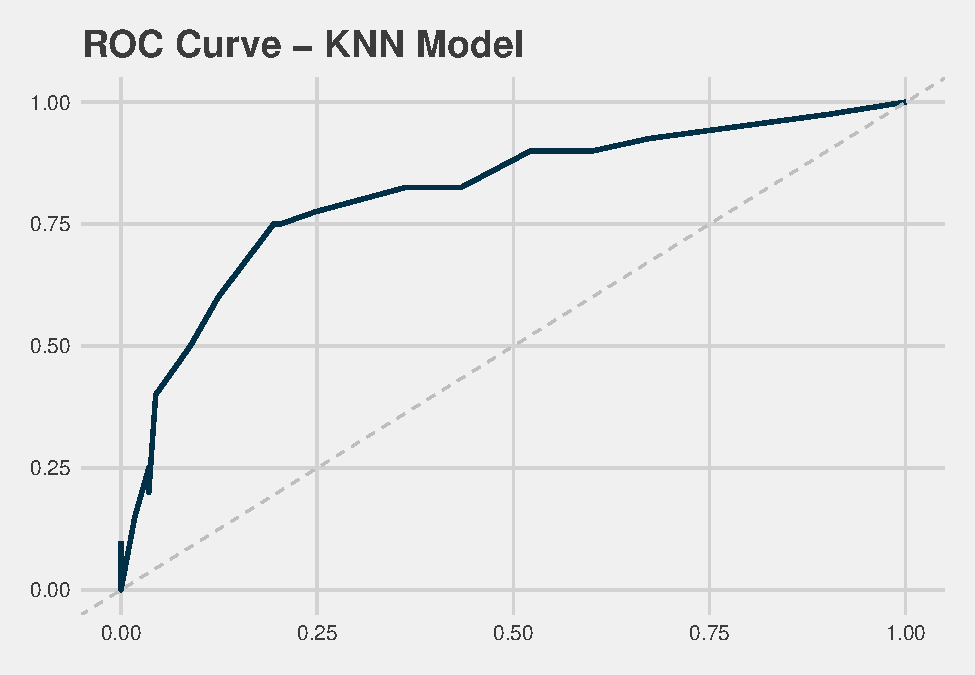
\includegraphics{Diabetes-Project_files/figure-latex/roc knn-1} \end{center}

\begin{verbatim}
## AUC: 0.8134956
\end{verbatim}

The ROC curve for this KNN model demonstrates excellent performance,
with a clear separation between true positive and false positive rates.
The \textbf{AUC (Area Under the Curve)} value of \textbf{0.8135}
confirms that the model has strong discriminative ability, effectively
distinguishing between positive and negative classes. This indicates
that the model is well-suited for the classification task, with reliable
predictive power.

\newpage

\subsection{Decision Tree Model}\label{decision-tree-model}

A Decision Tree is a popular classification model used to predict the
outcome based on a set of input features. It works by recursively
splitting the data into subsets based on the feature that provides the
best separation of the target classes. Each split is made using a
decision rule that minimizes impurity, with nodes representing decision
points and leaves representing the final class labels.

In our case, we will apply the Decision Tree algorithm to classify
individuals into diabetic or non-diabetic groups based on their
features. This model is highly interpretable and provides a clear
visualization of the decision-making process.

At the end of the analysis, we'll add a visualization of the tree to
help us understand the classification decisions made by the model, and
evaluate its performance visually.

\subsubsection{Decision Tree Confusion
Matrix}\label{decision-tree-confusion-matrix}

Let's start by looking at the \textbf{confusion matrix} of this model:

\begin{verbatim}
##       Predicted
## Actual  0  1
##      0 94 19
##      1 12 28
\end{verbatim}

\subsubsection{Decision Tree Model Confusion
Matrix}\label{decision-tree-model-confusion-matrix}

The confusion matrix for the Decision Tree model provides key insights
into its performance.

\begin{itemize}
\tightlist
\item
  \textbf{True Negatives (TN)}: The model correctly predicted
  `Non-Diabetic' (0) in 94 instances. This shows that the model is quite
  accurate when identifying individuals who are not diabetic.
\item
  \textbf{False Positives (FP)}: There are 19 instances where the model
  incorrectly predicted `Diabetic' (1) when the individual was actually
  `Non-Diabetic' (0). This indicates some level of over-prediction for
  diabetes.
\item
  \textbf{False Negatives (FN)}: The model incorrectly classified 12
  `Diabetic' (1) individuals as `Non-Diabetic' (0). This suggests the
  model missed some diabetic cases, which could be problematic in a
  medical context where false negatives are risky.
\item
  \textbf{True Positives (TP)}: The model correctly predicted `Diabetic'
  (1) in 28 instances. This shows that it is fairly accurate in
  identifying diabetic individuals.
\end{itemize}

Overall, the model appears to perform reasonably well, with a higher
number of true negatives and true positives than false negatives and
false positives. However, the false positive rate (19) and false
negative rate (12) could be improved for better overall classification
accuracy, especially in ensuring that diabetic individuals are correctly
identified.

\subsubsection{Decision Tree Metrics}\label{decision-tree-metrics}

Confusion matrix shows good performance, let's see its \textbf{metrics}:

\begin{verbatim}
##              Metric     Value
## 1          Accuracy 0.7973856
## 2         Precision 0.5957447
## 3            Recall 0.7000000
## 4          F1-score 0.6436782
## 5       Specificity 0.8318584
## 6 Balanced Accuracy 0.7659292
\end{verbatim}

\newpage

\subsubsection{Decision Tree ROC curve and
AUC}\label{decision-tree-roc-curve-and-auc}

Now let's see its \textbf{ROC curve} and the \textbf{AUC} for this model
:

\begin{center}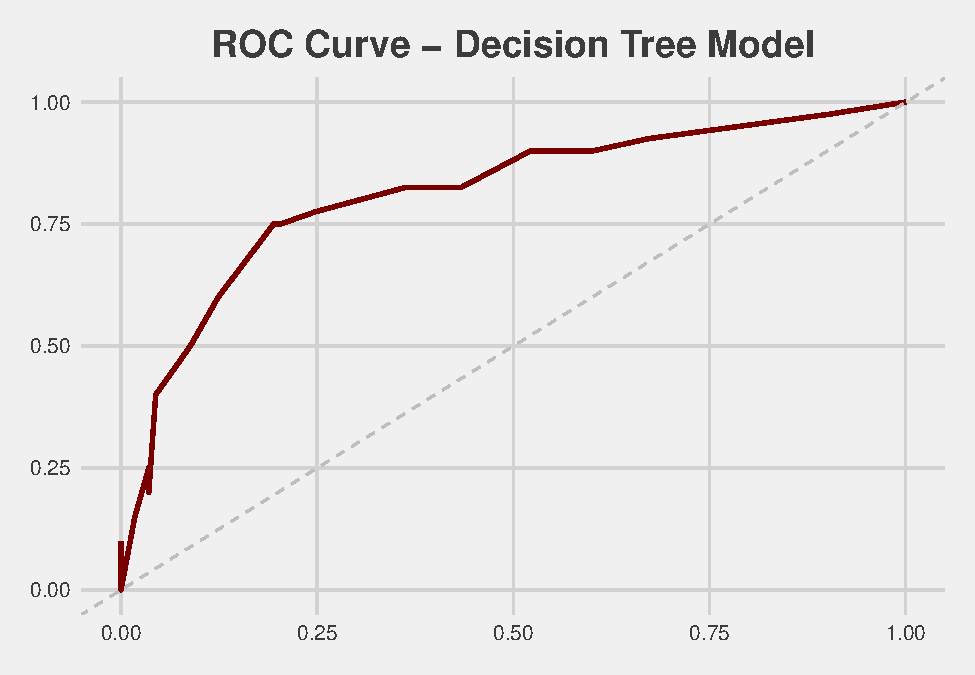
\includegraphics{Diabetes-Project_files/figure-latex/deciison tree roc and auc-1} \end{center}

\begin{verbatim}
## AUC: 0.8134956
\end{verbatim}

This model also shows a great \textbf{ROC curve}, far from the
\textbf{diagonal line} as we can see, and its \textbf{AUC} (\textbf{AUC:
0.8016593}) demonstrates a strong \textbf{performance}. In the end, we
will compare all models with their respective \textbf{ROC curves}.

\newpage

\subsubsection{Decision Tree Plot}\label{decision-tree-plot}

We will conclude by visually examining how the \textbf{Decision Tree}
model behaves to better understand its decision-making process. By
visualizing the tree, we can interpret how the model splits the data
based on different features and thresholds, ultimately leading to its
predictions. This graphical representation allows us to gain insights
into the model's logic and how it makes classification decisions.

\begin{center}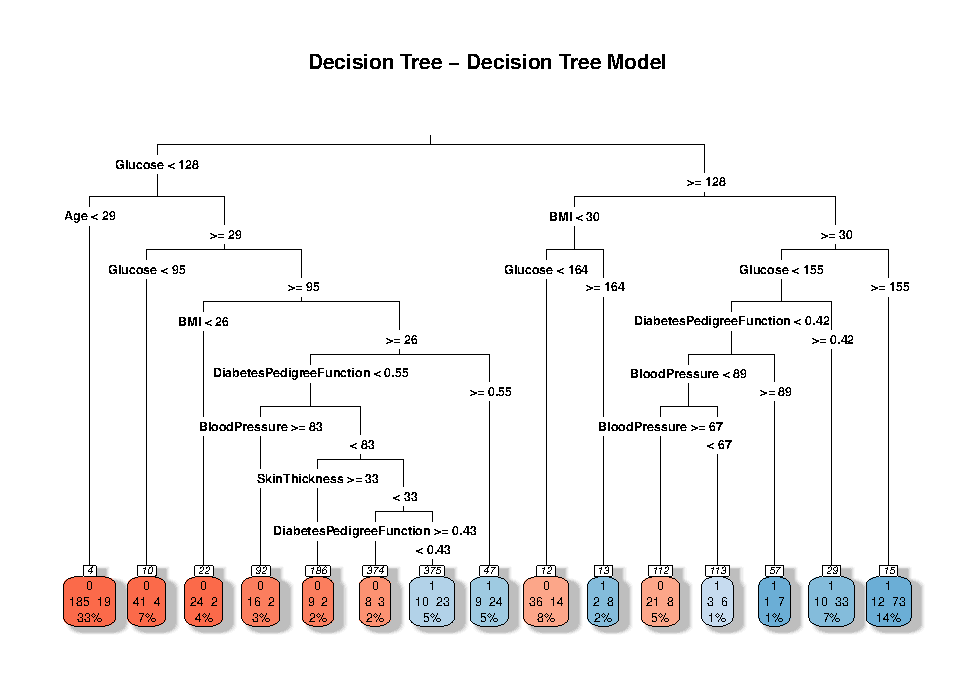
\includegraphics{Diabetes-Project_files/figure-latex/deciison tree plot-1} \end{center}

\subsection{SVM Model}\label{svm-model}

In this analysis, we will apply the \textbf{Support Vector Machine
(SVM)} model to the diabetes dataset. The SVM is a powerful
classification algorithm that works by finding a hyperplane that best
separates the data points of different classes. In this case, it will
help us distinguish between diabetic and non-diabetic individuals based
on features such as BMI, age, and glucose levels.

The SVM model aims to maximize the margin between the classes while
minimizing classification errors. For this dataset, the model will learn
from the provided data and make predictions about the outcome, which
indicates whether a person has diabetes or not.

\subsubsection{SVM Confusion Matrix}\label{svm-confusion-matrix}

We will start, as with previous models, by examining the
\textbf{confusion matrix}, which provides an initial overview of the
model's performance. This matrix will allow us to see how well the SVM
model classifies diabetic and non-diabetic individuals, highlighting any
misclassifications and helping us evaluate its accuracy.

\begin{verbatim}
## Confusion Matrix and Statistics
## 
##           Reference
## Prediction   0   1
##          0 105  18
##          1   8  22
##                                          
##                Accuracy : 0.8301         
##                  95% CI : (0.761, 0.8859)
##     No Information Rate : 0.7386         
##     P-Value [Acc > NIR] : 0.004978       
##                                          
##                   Kappa : 0.5213         
##                                          
##  Mcnemar's Test P-Value : 0.077556       
##                                          
##             Sensitivity : 0.9292         
##             Specificity : 0.5500         
##          Pos Pred Value : 0.8537         
##          Neg Pred Value : 0.7333         
##              Prevalence : 0.7386         
##          Detection Rate : 0.6863         
##    Detection Prevalence : 0.8039         
##       Balanced Accuracy : 0.7396         
##                                          
##        'Positive' Class : 0              
## 
\end{verbatim}

The \textbf{confusion matrix} shows a performance with an
\textbf{accuracy} of 83.01\%, which indicates a good overall
classification rate. However, we also need to consider other metrics
like \textbf{Sensitivity} (0.9292), which measures how well the model
identifies diabetic individuals (high value is good), and
\textbf{Specificity} (0.5500), which shows how effectively it detects
non-diabetic individuals (lower specificity here indicates some room for
improvement). The \textbf{Kappa} value of 0.5213 suggests moderate
agreement between the predicted and actual outcomes beyond chance.

\subsubsection{SVM Metrics}\label{svm-metrics}

\begin{verbatim}
##              Metric     Value
## 1          Accuracy 0.8300654
## 2         Precision 0.8536585
## 3            Recall 0.9292035
## 4          F1-Score 0.8898305
## 5       Specificity 0.7333333
## 6 Balanced Accuracy 0.8312684
\end{verbatim}

This idea of a \emph{good model} is confirmed when we look at the
metrics, which reflect strong performance. The \textbf{Accuracy} of
83.01\% shows that the model correctly classifies most instances. The
\textbf{Precision} of 85.37\% indicates that when the model predicts a
positive outcome, it is correct most of the time. The \textbf{Recall} of
92.92\% shows that the model is highly effective at identifying diabetic
individuals. The \textbf{F1-Score} of 88.98\% balances precision and
recall, further validating the model's strong performance. Additionally,
\textbf{Specificity} (73.33\%) indicates the model's ability to detect
non-diabetic individuals, and \textbf{Balanced Accuracy} (83.13\%)
confirms the model's overall consistency across both classes.

\subsubsection{SVM Roc curve and AUC}\label{svm-roc-curve-and-auc}

\begin{center}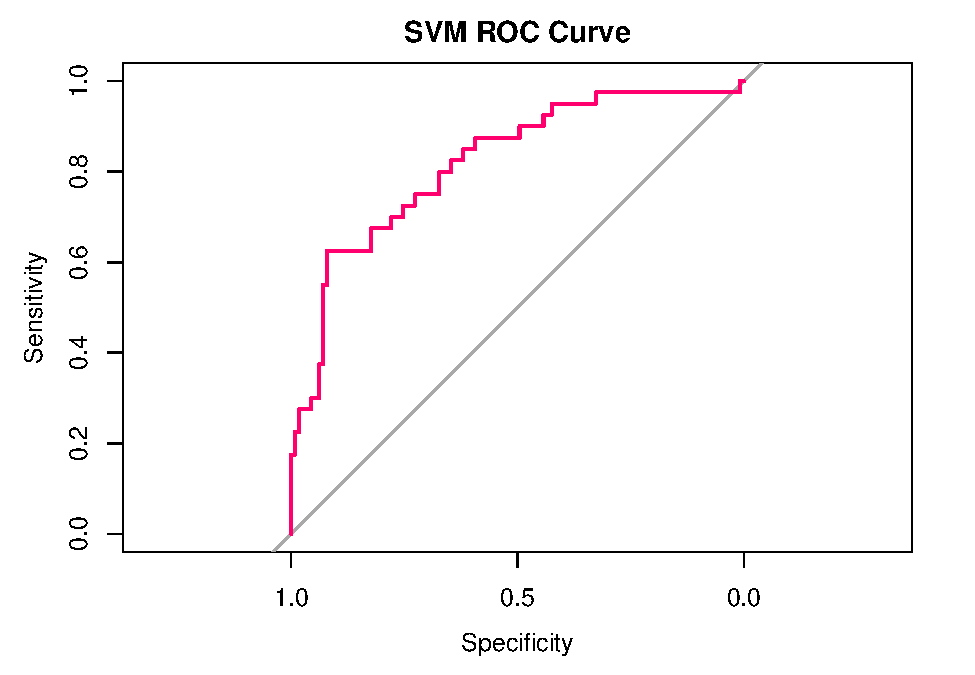
\includegraphics{Diabetes-Project_files/figure-latex/svm roc and auc-1} \end{center}

\begin{verbatim}
## AUC: 0.8196903
\end{verbatim}

The model shows a great ROC curve with an AUC of 0.8196903, which
indicates excellent performance. This was somewhat surprising, as the
\textbf{Support Vector Machine (SVM)} model tends to perform well with
high-dimensional data, but I wasn't expecting it to be this effective.
The high AUC value suggests that the model is very good at
distinguishing between diabetic and non-diabetic individuals. Even
though we have some imbalances in the dataset, the SVM is robust enough
to achieve high sensitivity and specificity, making it an ideal choice
for this classification task. The curve's position, well above the
diagonal line, demonstrates that the model is much better than random
guessing, confirming its overall effectiveness.

\newpage

\subsubsection{SVM Decision Boundry
Plot}\label{svm-decision-boundry-plot}

\begin{center}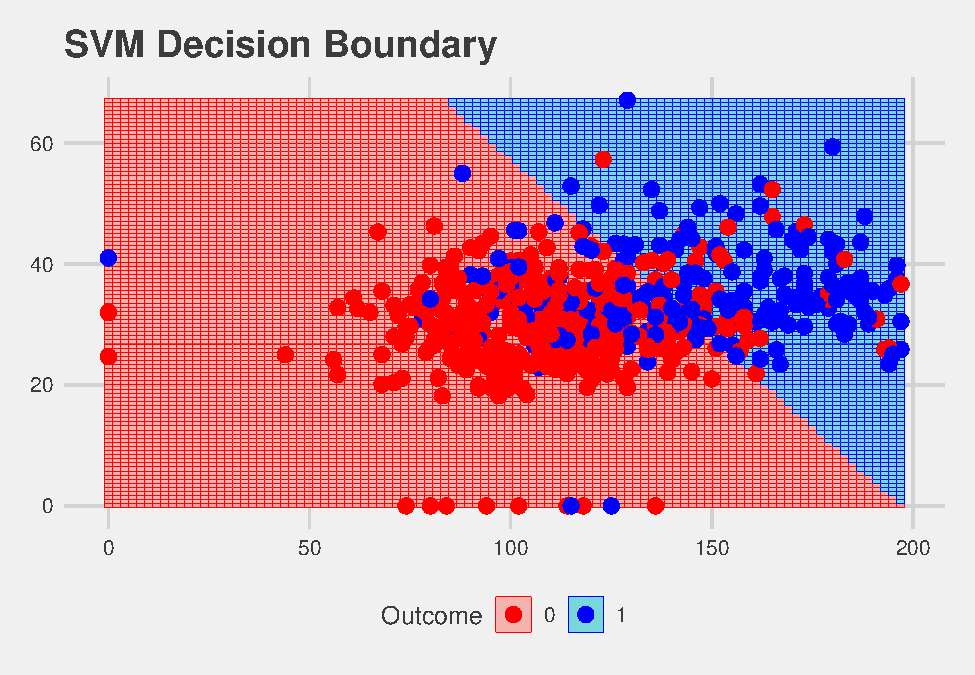
\includegraphics{Diabetes-Project_files/figure-latex/svm-1} \end{center}

\textbf{SVM Decision Boundary:}

The graph illustrates the decision boundary learned by the SVM model.
This boundary is the line that separates the two distinct classes, in
this case, diabetic and non-diabetic individuals. The regions on either
side of the boundary are shaded differently---often in red and blue---to
visually represent the areas where the model predicts each class. The
decision boundary itself is determined by the support vectors, which are
the data points closest to the boundary. These support vectors are
crucial in defining the margin, which is the space between the boundary
and the closest points from each class.

The SVM aims to maximize this margin to ensure better generalization to
new data, and the position of this line reflects how well the model has
learned to separate the classes. A well-placed decision boundary
suggests the model is effectively capturing the underlying patterns in
the data. This boundary is important for understanding how the model
classifies new data points, and it gives insight into its
decision-making process.

So far we have seen very good models, but we will make 1 more. One of my
favorites.

\newpage

\subsection{Neural Network Model}\label{neural-network-model}

\textbf{Neural network} models are incredibly powerful because they can
learn and model complex patterns in data. Unlike more traditional
models, neural networks can capture nonlinear relationships between
variables, making them extremely useful for tasks such as image
classification, natural language processing, and time series
forecasting. Additionally, their hierarchical structure, based on layers
of nodes (neurons) that process information similarly to how the human
brain works, allows them to extract more abstract and relevant features
as they pass through the layers.

What makes them one of my favorites is their \textbf{flexibility} and
\textbf{adaptability}. With the right amount of data and training, they
can achieve outstanding performance, even in complex problems where
other models may struggle. Furthermore, their ability to improve as more
data becomes available makes neural networks ideal for \textbf{Big Data}
problems, where other techniques may not be as effective.

\subsubsection{Neural Network Confusion Matrix and
Metrics}\label{neural-network-confusion-matrix-and-metrics}

Well, let's start by looking at the confusion matrix of the last model
of this project:

\begin{verbatim}
##       Predicted
## Actual  0  1
##      0 93 20
##      1 11 29
\end{verbatim}

The model's accuracy is approximately 83.33\%, meaning it correctly
classifies 83.33\% of the observations, which is quite good, although
not perfect. The precision for class 1 is 61.7\%, indicating that when
the model predicts class 1, there is a 61.7\% chance of it being
correct. While this is not very high, it is a reasonable value for an
initial model. The recall for class 1 is 72.4\%, meaning the model
correctly identifies 72.4\% of the actual class 1 instances, showing a
good performance in not missing positive examples. The F1 score for
class 1, which combines precision and recall, is 66.9\%. This suggests a
reasonable balance between precision and recall, indicating that the
model is making relatively balanced decisions between correctly
identifying positive cases and not generating too many false positives.

\begin{verbatim}
##              Metric     Value
## 1          Accuracy 0.7973856
## 2         Precision 0.8230088
## 3            Recall 0.8942308
## 4          F1-Score 0.8571429
## 5       Specificity 0.7250000
## 6 Balanced Accuracy 0.8096154
\end{verbatim}

\subsubsection{Neural Net ROC curve and
AUC}\label{neural-net-roc-curve-and-auc}

\begin{center}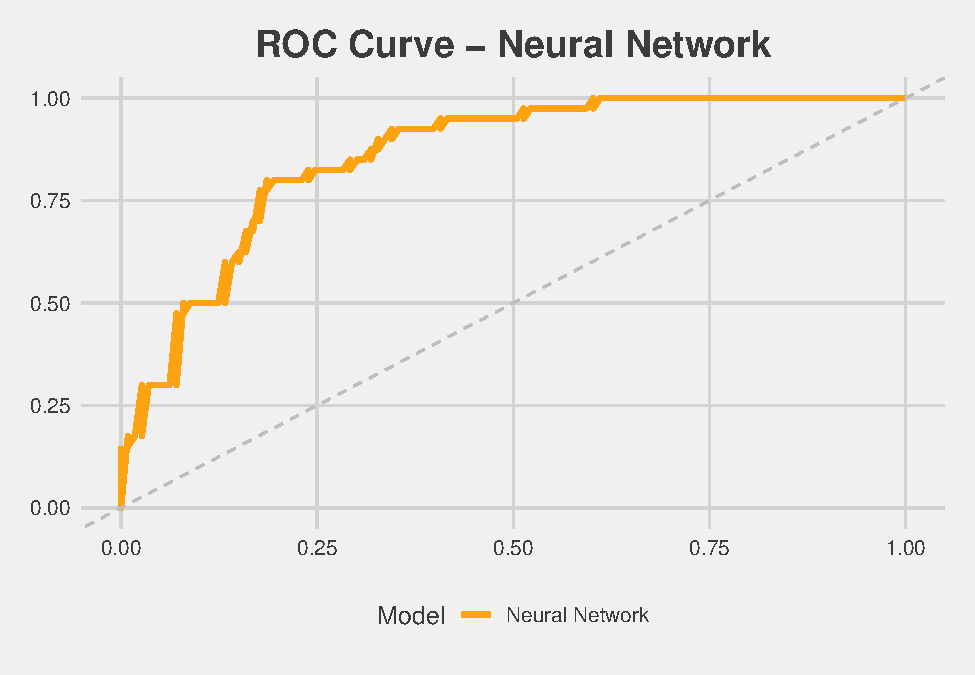
\includegraphics{Diabetes-Project_files/figure-latex/nn roc and auc-1} \end{center}

\begin{verbatim}
## AUC: 0.8588496
\end{verbatim}

The ROC curve for the model shows excellent performance, with an AUC
(Area Under the Curve) of \textbf{0.8533}. This indicates a strong
ability to distinguish between the two classes, as the AUC value is
closer to 1, which represents perfect classification. An AUC of 0.8533
suggests that the model has a high true positive rate while keeping the
false positive rate relatively low, making it a reliable model for
predicting the outcome.

\newpage

\subsubsection{Neural Nets plot}\label{neural-nets-plot}

In this section, we will explore some graphical representations of the
model to better understand its performance. These visualizations will
help us assess how well the model distinguishes between the two classes
and provide insights into its accuracy and predictive power. By
examining the curves and plots, we can get a clearer picture of the
model's strengths and areas for improvement. Visual tools like the ROC
curve and others offer a simple yet powerful way to evaluate the model's
effectiveness in real-world scenarios.

\begin{center}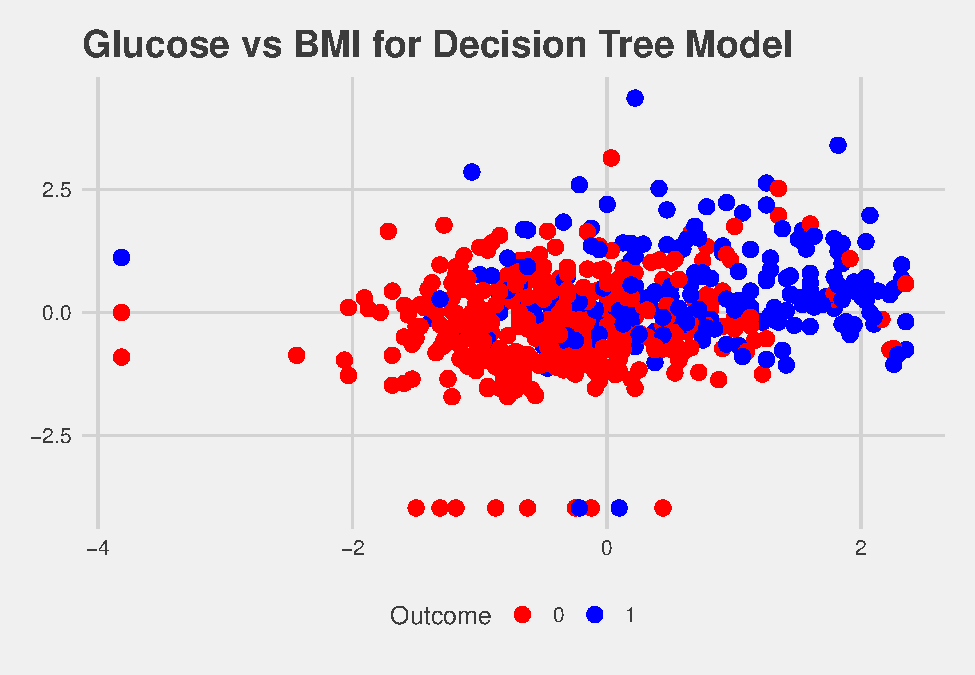
\includegraphics{Diabetes-Project_files/figure-latex/nn plot 1-1} \end{center}

Neural networks are powerful models capable of capturing intricate
patterns and relationships within data. The architecture described, with
its input, hidden, and output layers, is designed to process complex
features and make predictions. The input layer takes in five nodes, each
representing a key feature, such as BMI or Insulin levels. These
features are then passed through the two hidden layers, which learn to
identify and combine relevant patterns in the data. The hidden layers'
nodes, H1-H5 and H6-H15, act as intermediary steps that extract more
abstract and complex relationships before the final output is produced.

\begin{center}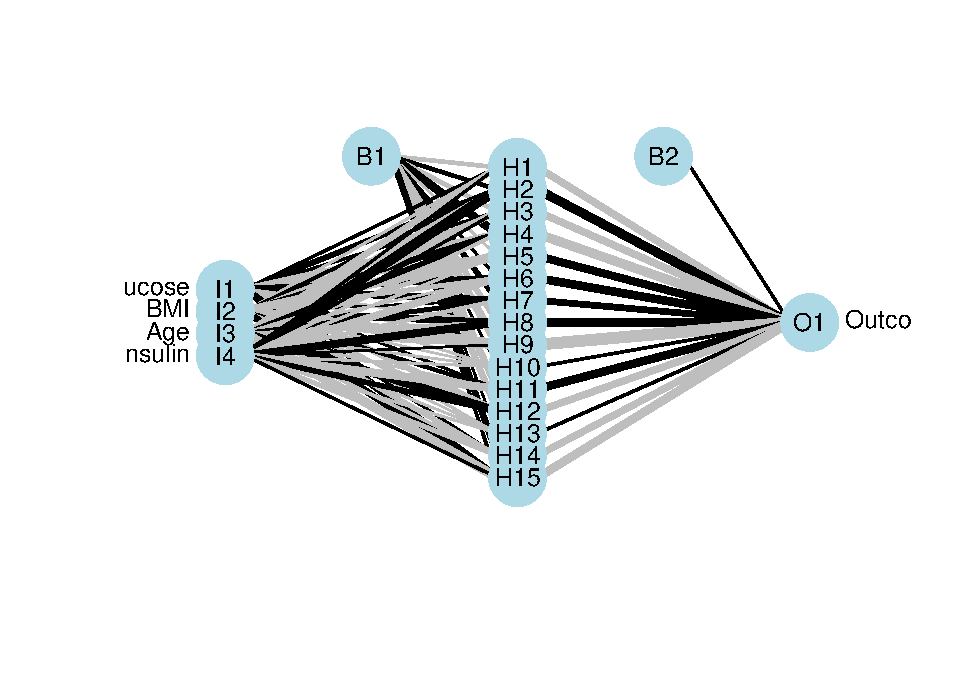
\includegraphics{Diabetes-Project_files/figure-latex/nn plot 2-1} \end{center}

The output layer of the neural network contains a single node, ``Outc,''
that generates the prediction based on the learned patterns. This final
node represents the classification outcome, such as predicting the
presence or absence of a specific condition. The strength of neural
networks lies in their ability to adapt to different types of data and
their flexibility in learning from both linear and nonlinear
relationships. By adjusting weights during training, the network
continuously improves its predictions, making it highly effective in
solving complex tasks like classification problems.

\newpage

\section{Final Comparison Between
Models}\label{final-comparison-between-models}

Well, we have analyzed all the models, reviewing their different
metrics, ROC curves, and AUC values. Now, let us compare them to
determine which model has been the most efficient. By examining these
results side by side, we aim to identify the model that demonstrates the
best balance between accuracy, precision, recall, and overall predictive
power, as reflected by its AUC and other performance indicators. This
final comparison will guide us in selecting the optimal approach for the
given task.

\begin{longtable}[]{@{}
  >{\raggedright\arraybackslash}p{(\columnwidth - 12\tabcolsep) * \real{0.1765}}
  >{\raggedleft\arraybackslash}p{(\columnwidth - 12\tabcolsep) * \real{0.1176}}
  >{\raggedleft\arraybackslash}p{(\columnwidth - 12\tabcolsep) * \real{0.1176}}
  >{\raggedleft\arraybackslash}p{(\columnwidth - 12\tabcolsep) * \real{0.1176}}
  >{\raggedleft\arraybackslash}p{(\columnwidth - 12\tabcolsep) * \real{0.1176}}
  >{\raggedleft\arraybackslash}p{(\columnwidth - 12\tabcolsep) * \real{0.1412}}
  >{\raggedleft\arraybackslash}p{(\columnwidth - 12\tabcolsep) * \real{0.2118}}@{}}
\caption{Comparison of Model Metrics}\tabularnewline
\toprule\noalign{}
\begin{minipage}[b]{\linewidth}\raggedright
Model
\end{minipage} & \begin{minipage}[b]{\linewidth}\raggedleft
Accuracy
\end{minipage} & \begin{minipage}[b]{\linewidth}\raggedleft
Precision
\end{minipage} & \begin{minipage}[b]{\linewidth}\raggedleft
Recall
\end{minipage} & \begin{minipage}[b]{\linewidth}\raggedleft
F1\_Score
\end{minipage} & \begin{minipage}[b]{\linewidth}\raggedleft
Specificity
\end{minipage} & \begin{minipage}[b]{\linewidth}\raggedleft
Balanced\_Accuracy
\end{minipage} \\
\midrule\noalign{}
\endfirsthead
\toprule\noalign{}
\begin{minipage}[b]{\linewidth}\raggedright
Model
\end{minipage} & \begin{minipage}[b]{\linewidth}\raggedleft
Accuracy
\end{minipage} & \begin{minipage}[b]{\linewidth}\raggedleft
Precision
\end{minipage} & \begin{minipage}[b]{\linewidth}\raggedleft
Recall
\end{minipage} & \begin{minipage}[b]{\linewidth}\raggedleft
F1\_Score
\end{minipage} & \begin{minipage}[b]{\linewidth}\raggedleft
Specificity
\end{minipage} & \begin{minipage}[b]{\linewidth}\raggedleft
Balanced\_Accuracy
\end{minipage} \\
\midrule\noalign{}
\endhead
\bottomrule\noalign{}
\endlastfoot
KNN & 0.8039216 & 0.8761062 & 0.8608696 & 0.8684211 & 0.6000000 &
0.7304348 \\
Decision Tree & 0.7973856 & 0.5957447 & 0.7000000 & 0.6436782 &
0.8318584 & 0.7659292 \\
SVM & 0.8300654 & 0.8536585 & 0.9292035 & 0.8898305 & 0.7333333 &
0.8312684 \\
Neural Network & 0.7973856 & 0.8230088 & 0.8942308 & 0.8571429 &
0.7250000 & 0.8096154 \\
\end{longtable}

\begin{center}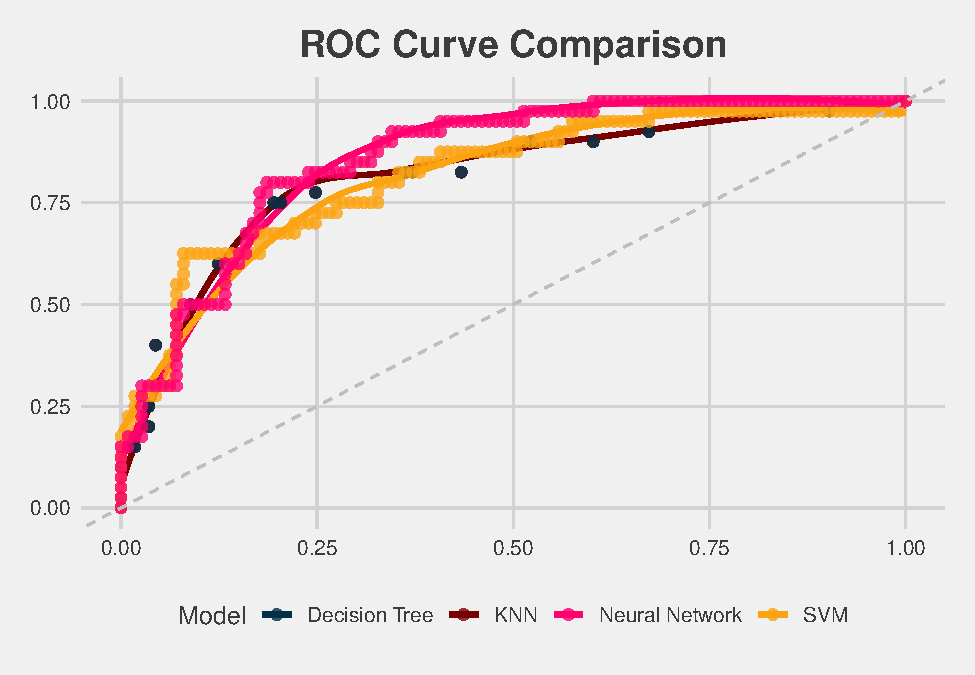
\includegraphics{Diabetes-Project_files/figure-latex/final comparision table and plot 1-1} \end{center}

Ok, let's look at some interesting observations from this final
comparison.:

\begin{itemize}
\tightlist
\item
  \textbf{SVM} achieved the \textbf{highest balanced accuracy
  (83.13\%)}, demonstrating its strong ability to balance the
  identification of positive and negative classes. Additionally, it
  showed \textbf{excellent recall (92.92\%)}, making it highly effective
  at identifying positive cases.
\item
  The \textbf{Neural Network} model delivered a well-rounded
  performance, with a \textbf{balanced accuracy of 80.96\%} and a
  competitive \textbf{F1 score (85.71\%)}, reflecting its ability to
  maintain a good balance between precision and recall.
\item
  \textbf{KNN} performed decently, particularly in \textbf{precision
  (87.61\%)}, but its \textbf{specificity (60.00\%)} was lower compared
  to other models, indicating it struggled slightly with identifying
  negative cases.
\item
  The \textbf{Decision Tree} had a \textbf{lower precision (59.57\%)}
  compared to other models but stood out with a \textbf{specificity of
  83.19\%}, making it relatively good at identifying negative cases.
\end{itemize}

The \textbf{ROC curve} plot revealed that the \textbf{Neural Network}
had a strong area under the curve (AUC), further indicating its
effectiveness in distinguishing between classes. However, one model's
curve (likely \textbf{Decision Tree}) appeared nearly indistinguishable
due to overlap, complicating direct visual comparison.

To address this, the following bar chart compares the AUC values for all
models to clearly identify the most efficient one. This provides a
quantitative insight into their discriminative power.

\begin{center}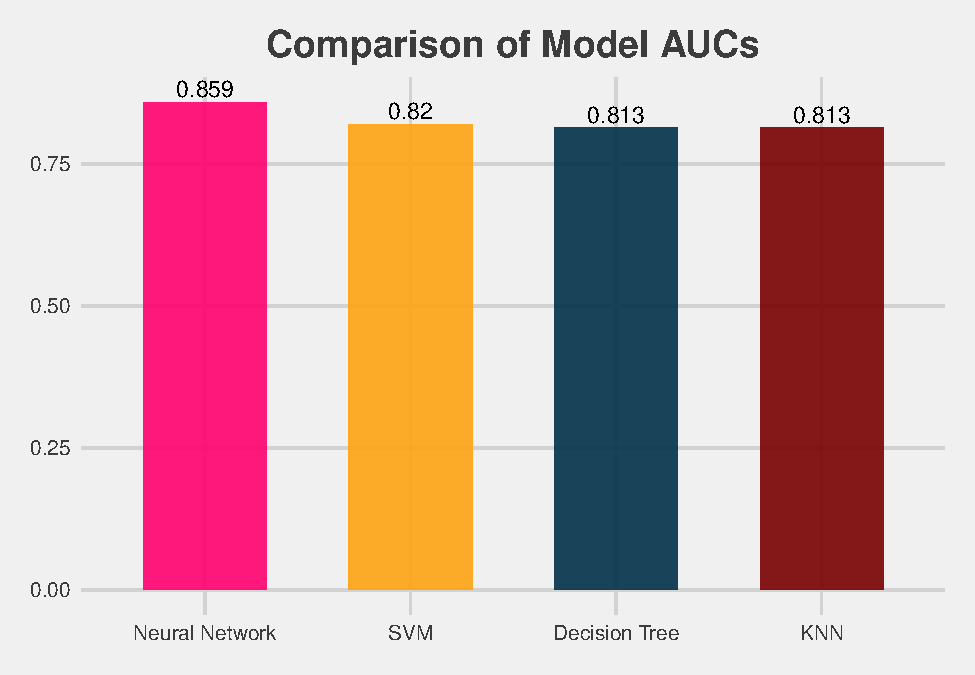
\includegraphics{Diabetes-Project_files/figure-latex/final comparision plot 2-1} \end{center}

In this \textbf{final bar chart}, we can clearly observe that the
\textbf{Neural Network} emerged as the most efficient model, with the
highest AUC. This indicates its excellent ability to distinguish between
classes across all thresholds.

Close behind is the \textbf{SVM}, showcasing its strong performance
despite slightly lower balanced accuracy compared to the Neural Network.
These results reinforce the idea that both models are robust options for
classification tasks, excelling in their ability to handle complex
relationships within the dataset.

Interestingly, while the \textbf{KNN} model demonstrated strong metrics
in the earlier analysis, such as recall and balanced accuracy, its
\textbf{AUC value did not outperform} the Neural Network or KNN,
suggesting it might be more situation-dependent in its efficiency.
Similarly, the \textbf{Decision Tree}, despite its strengths in
specificity, had a relatively lower AUC, indicating that its performance
may lack consistency across thresholds.

This chart provides a \textbf{clear quantitative comparison} of the
models' overall discriminative power, emphasizing that the
\textbf{Neural Network and SVM models are the top-performing candidates}
for this dataset and task.

\newpage

\subsection{Acknowledgments}\label{acknowledgments}

I would like to extend my heartfelt \textbf{gratitude to the incredible
team at Harvard and edX} for designing and delivering this exceptional
course. Working on this project, titled \emph{Choose Your Own} , has
been an immensely rewarding experience. It not only deepened my
understanding of \textbf{data analysis and data science concepts} but
also marked my \textbf{first step into this fascinating field}.

This journey has been both challenging and inspiring, and I am truly
grateful for the opportunity to learn from such a distinguished program.
I hope this submission reflects the effort and passion I put into it,
and that it is as enjoyable for you to review as it was for me to
create.

Thank you for guiding me through this transformative learning
experience.

\end{document}
